\subsection{\texorpdfstring{\(p\) -th power integrable functions}{p -th power integrable functions}}

The vector space \(\mathcal{K}(X;F)\) (which we shall denote simply by \(K_{F}\) if there is no fear of confusion), consisting of the continuous functions of X into F with compact support, is obviously a subspace of each of the vector spaces \(F_{F}^{p}\) .

DEFINITION 2. --- Given a locally compact space X, a measure \(\mu\) on X, and a Banach space F, we denote by \(\mathcal{L}_{\mathrm{F}}^{p}(\mathrm{X},\mu)\) (or simply \(\mathcal{L}_{\mathrm{F}}^{p}(\mu)\) , or \(\mathcal{L}_{\mathrm{F}}^{p}\) ) the closure, in the locally convex space \(\mathcal{F}_{\mathrm{F}}^{p}(\mathrm{X},\mu)\) , of the vector space \(\mathcal{K}(\mathrm{X};\mathrm{F})\) of continuous mappings of X into F with compact support. We denote by \(\mathrm{L}_{\mathrm{F}}^{p}(\mathrm{X},\mu)\) (or \(\mathrm{L}_{\mathrm{F}}^{p}(\mu)\) , or \(\mathrm{L}_{\mathrm{F}}^{p}\) ) the (normed) Hausdorff space associated with \(\mathcal{L}_{\mathrm{F}}^{p}(\mathrm{X},\mu)\) . The functions belonging to \(\mathcal{L}_{\mathrm{F}}^{p}\) are called the \(p\) -th power integrable functions (*).

Obviously \(\mathcal{L}_{\mathrm{F}}^{p}(\mathrm{X},|\mu |) = \mathcal{L}_{\mathrm{F}}^{p}(\mathrm{X},\mu)\) and \(\mathrm{L}_{\mathrm{F}}^{p}(\mathrm{X},|\mu |) = \mathrm{L}_{\mathrm{F}}^{p}(\mathrm{X},\mu)\) .

We shall write \(L^{p}\) and \(L^{p}\) instead of \(L_{R}^{p}\) and \(L_{R}^{p}\) (or of \(L_{C}^{p}\) and \(L_{C}^{p}\) when this causes no confusion). If F is a complex Banach space, \(L_{F}^{p}\) and \(L_{F}^{p}\) are equipped with the structure of a topological vector space over the field C (No.~3, Remark).

It is clear that every function in \(F_{F}^{p}\) that is equivalent to a function in \(L_{F}^{p}\) , belongs to \(L_{F}^{p}\) . A function with values in F and defined almost everywhere in X is again said to be p-th power integrable if it is equivalent to a function in \(L_{F}^{p}\) ; similarly a function with values in \(\overline{R}\) , defined and finite almost everywhere in X, is said to be p-th power integrable if it is equivalent to a function in \(L^{p}\) .

The functions in \(L_{F}^{p}\) (resp. in \(L^{p}\) ) are thus the p-th power integrable functions that are defined on all of X (resp. defined and finite on all of X). In this section and the following one, most of the propositions proved for the functions in \(L_{F}^{p}\) (resp. \(L^{p}\) ) may immediately be extended to p-th power integrable functions that are not everywhere defined (resp. that are not everywhere defined and finite); we shall usually leave to the reader the task of formulating and proving these results.

Remarks. --- 1) As has already been signalled (§2, No.~5) the p-th power integrable functions with values in F in general do not form a vector space.

\begin{enumerate}
\def\labelenumi{\arabic{enumi})}
\setcounter{enumi}{1}
\tightlist
\item
  In general, the space \(\mathcal{F}_{\mathrm{F}}^{p}\) is distinct from its subspace \(\mathcal{L}_{\mathrm{F}}^{p}\) (§4, Exer. 8).
\end{enumerate}

Def. 2 immediately yields the following criterion:

PROPOSITION 7. --- For a function f to belong to \(L_{F}^{p}\) , it is necessary and sufficient that, for every \(\varepsilon > 0\) , there exist a continuous function g with compact support such that \(\mathrm{N}_{p}(\mathbf{f} - \mathbf{g}) \leqslant \varepsilon\) .

In other words, the functions in \(L_{F}^{p}\) are the limits of sequences of continuous functions with compact support, for the topology of convergence in mean of order p.

PROPOSITION 8. --- Let f be a numerical function (finite or not) defined almost everywhere; if, for every \(\varepsilon > 0\) , there exists two p-th power integrable functions g, h such that \(g \leqslant f \leqslant h\) almost everywhere and \(\mathrm{N}_{p}(h - g) \leqslant \varepsilon\) , then f is p-th power integrable.

For, \(f\) is finite almost everywhere and \(\mathrm{N}_p(f - g) \leqslant \mathrm{N}_p(h - g) \leqslant \varepsilon\) ; Prop. 7 therefore shows that \(f\) is \(p\) -th power integrable.

Since, by definition, \(L_{F}^{p}\) is a closed subspace of \(F_{F}^{p}\) , and since the latter space is complete (No.~3, Prop. 5), we have the following result (GT, II, §3, No.~4, Prop. 8):

THEOREM 2. --- The space \(\mathcal{L}_{\mathrm{F}}^{p}\) is complete; the space \(\mathrm{L}_{\mathrm{F}}^{p}\) is a Banach space.

In the space \(L_{F}^{p}\) , the norm \(\mathrm{N}_{p}(\widetilde{\mathbf{f}})\) of a class is again denoted \(\| \widetilde{f} \|_{p}\) .

Th. 2 can be sharpened as follows:

THEOREM 3. --- Let \((\mathbf{f}_n)\) be a Cauchy sequence in the space \(\mathcal{L}_{\mathrm{F}}^p\) ; there exists a subsequence \((\mathbf{f}_{n_k})\) of \((\mathbf{f}_n)\) having the following properties:

\(1^{\circ}\) the series with general term \(\mathrm{N}_p(\mathbf{f}_{n_{k + 1}} - \mathbf{f}_{n_k})\) is convergent;

\(2^{\circ}\) the series with general term \(\mathbf{f}_{n_{k+1}}(x) - \mathbf{f}_{n_k}(x)\) is absolutely convergent almost everywhere;

\(3^{\circ}\) if \(\mathbf{f}\) is a function defined on X and equal almost everywhere to the limit of the sequence \((\mathbf{f}_{n_k}(x))\) , then \(\mathbf{f}\) belongs to \(\mathcal{L}_{\mathrm{F}}^p\) and the sequence \((\mathbf{f}_n)\) converges in mean of order \(p\) to \(\mathbf{f}\) ;

\(4^{\circ}\) there exists a lower semi-continuous function \(g \geqslant 0\) such that \(\mathrm{N}_p(g) < +\infty\) and such that, for every \(k\) , \(|\mathbf{f}_{n_k}(x)| \leqslant g(x)\) for all \(x \in X\) .

As in the proof of Prop. 5 of No.~3, it suffices to define the sequence \((n_k)\) by induction, in such a way that \(\mathrm{N}_p(\mathbf{f}_{n_{k+1}} - \mathbf{f}_{n_k}) \leqslant 2^{-k}\) ; parts \(2^\circ\) and \(3^\circ\) then follow from Prop. 6 of No.~3 and the fact that \(\mathcal{L}_{\mathrm{F}}^p\) is closed in \(\mathcal{F}_{\mathrm{F}}^p\) . On the other hand, if \(h(x)\) is the sum of the series with general term \(|\mathbf{f}_{n_{k+1}}(x) - \mathbf{f}_{n_k}(x)|\) , Th. 1 of No.~2 shows that \(\mathrm{N}_p(h) < +\infty\) ; therefore, by the definition of \(|\mu|^*\) , there exists a lower semi-continuous function \(g \geqslant h + |\mathbf{f}_{n_1}|\) such that \(\mathrm{N}_p(g) < +\infty\) , which completes the proof.

COROLLARY 1. --- If a Cauchy sequence \((\mathbf{f}_{n})\) in the space \(L_{F}^{p}\) is such that the sequence \((\mathbf{f}_{n}(x))\) converges almost everywhere to \(\mathbf{f}(x)\) , then f is p-th power integrable and the sequence \((\mathbf{f}_{n})\) converges in mean of order p to f.

For, there exists a subsequence \((\mathbf{f}_{n_{k}})\) of \((\mathbf{f}_{n})\) such that \((\mathbf{f}_{n_{k}}(x))\) converges almost everywhere to \(\mathbf{g}(x)\) , where g is a function in \(L_{F}^{p}\) such that \((\mathbf{f}_{n})\) converges in mean of order p to g. The hypotheses therefore imply that \(\mathbf{f}(x)=\mathbf{g}(x)\) almost everywhere, whence the corollary.

COROLLARY 2. --- Let E be a dense subset of \(L_{F}^{p}\) . For every function \(f \in L_{F}^{p}\) , there exists a sequence \((\mathbf{g}_{n})\) of functions in E having the following properties:

\(1^{\circ}\) the sequence \((\mathbf{g}_n)\) converges in mean of order \(p\) to \(\mathbf{f}\) ;

\(2^{\circ}\) for almost every \(x \in \mathbf{X}\) , the sequence \((\mathbf{g}_n(x))\) converges to \(\mathbf{f}(x)\) .

For, since the space \(L_{F}^{p}\) is metrizable, there exists a Cauchy sequence \((\mathbf{f}_{n})\) in \(L_{F}^{p}\) consisting of functions in E and convergent in mean of order p to f (GT, IX, §2, No.~6, Prop. 8); it suffices to apply Th. 3 to this sequence.

Cor. 2 is applicable in particular to the case where E is taken to be the space \(K_{F}\) of continuous functions with compact support.

\pandocbounded{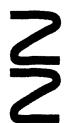
\includegraphics[keepaspectratio]{images/part001_fce77adb.jpg}}

Remarks. --- 1) A Cauchy sequence \((\mathbf{f}_n)\) in \(\mathcal{L}_{\mathrm{F}}^{p}\) can be such that the sequence \((\mathbf{f}_n(x))\) is not convergent at any point of X (Exer. 1).

\begin{enumerate}
\def\labelenumi{\arabic{enumi})}
\setcounter{enumi}{1}
\tightlist
\item
  If \(\mathbf{f}\) belongs to \(\mathcal{L}_{\mathrm{F}}^{p}\) , it is not always possible to find a sequence \((\mathbf{f}_n)\) of continuous functions with compact support such that the sequence \((\mathbf{f}_n(x))\) converges everywhere in \(X\) to a function equal to \(\mathbf{f}(x)\) almost everywhere (§4, Exer. 4 c)).
\end{enumerate}

